\chapter{Implementation: Dapp}
\section{DALICC}
According to [], DALICC stands for Data Licenses Clearance Center. It is software framework that helps people to legally secure data from third party and help to detect licensing conflicts and reducing the costs of rights clearance by enabling automated clearance right in creation of derivative works. 
\subsection{DALICC Requirements}
The following requirements would be addressed by DALICC framework:\\
\begin{itemize}
	\item \textit{Tackling license heterogeneity:} \\
	It is possible to combine the various contents which having the same license with different names. But that would be much difficult to license the resultant of the combined contents. To solve this issue, DALICC provides set of machine-readable representation of licenses that allow to compare licenses to each other to identify the equivalent licenses. It guides the user to possible conflicts of various combined licenses.
	\item \textit{Tackling REL heterogeneity:} \\
	Combing licenses are simple, if they are express through the same RED. But, it is difficult to compare licenses have been represented by different RELs.\\
	DALICC resolve this problem, by representing RELs based on semantic web, map the terms to each other. It will represent exiting RELs based on  W3C-approved standards, thus allow mapping between various RELs to be created.
	\item \textit{Compatibility check, conflict detection and neutrality of the rules:} \\
	It is difficult to be sure, if the meaning of the different terms in semantic are aligned. This problems result from indicating the classes, instances and properties which can not be handled just by mapping.\\
	This is where DALICC comes to play and helps user with a workflow that define the usage context, then gathering additional information to detect conflicts and ambiguous concepts. Based on this information, DALICC make reasoning over the set of licenses and infers the instruction to user how to process with license processing.\\
	\item \textit{Legal validity of representations and machine recommendations:} \\
	According to Anna Fensel\cite{Anna}, The semantic complexity of licensing issues means that the semantics of RELs must be clearly aligned within the specific application scenario. This includes a correct interpretation of the various national legislations according to the country of origin of a jurisdiction (i.e. German Urheberrecht vs. US copyright), the resolution of problems that are derived from multilinguality and the consideration of existing case law in the resolution of licensing conflicts.\cite{Anna}\\
	To solve this problem, DALICC will check the legal validity of machine-readable license and compatibility of reasoning engine output with law. DALICC output will be testes against law and checked the semantic precision of derived from different language and adjusted them.
	
\end{itemize}
\subsection{DALICC Software Architecture}
To address the above challenges DALICC framework consist of four components:\\
\begin{itemize}
	\item \textbf{License composer} is tools that allowed the license to be created from set of questions which are mapped to ODRL, ccREL and the DALICC vocabularies and concepts.
	\item \textbf{License library} is a repository that represents licenses in machine-readable format , the former as ORDL policies and the letters as plain text.
	\item \textbf{License annotator} allows to attache license to dataset, either by choosing available licenses in license library or create new license using license composer.
	\item \textbf{License negotiator} as main component in DALICC framework that checks the license compatibility and support license conflicts by detecting equivalence license having various names.
\end{itemize}
\begin{center}
	
	\begin{figure}[htb!]
		
		\begin{minipage}{0.75\linewidth}
			
			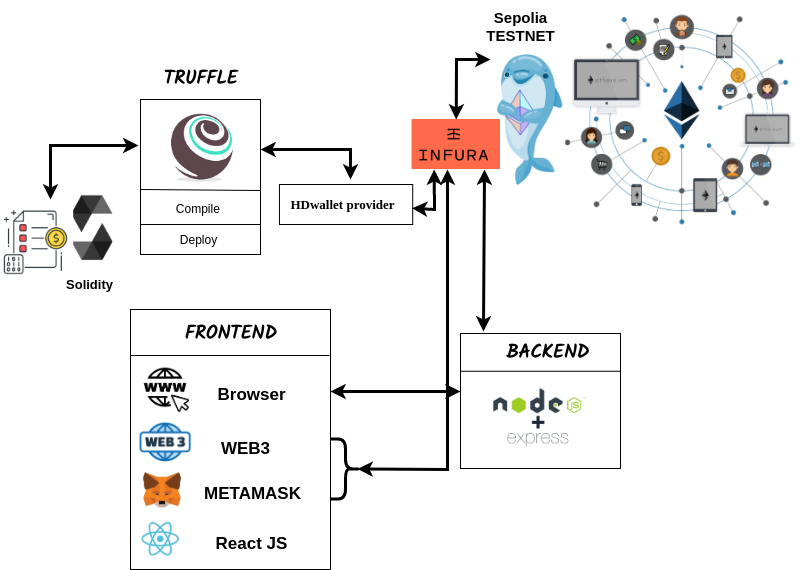
\includegraphics[width=1.45\textwidth]{images/chap03_dapp.png}
		\end{minipage}
		\caption{DApp infrastructure}
		
	\end{figure}
	
\end{center}
\section{Project Concepts}

In this section, we focused on requirements that we need to address them in our application.
And some terms that we mostly heard of them in smart contract section.\\
\textbf{Triple} use as template in this project. it contains different \\ concepts likr class and properties associated with project transaction graph.\\
\textbf{SPARQL} is language query that runs over tripled produced by ...\\

\textbf{Http Request} 
\subsection{Contract and Ontology specification}
Here, it is explained some terms related to smart contract and ontology of our application. And we needed them as primary requirement to build up this dApp.
\begin{itemize}
	\item \textbf{Definition 1 (Owner)} is the address of deployed contract or transaction to the blockchain. that is the first msg sender to interact with contract. In this caseed is able to change her/his license of the file.\\
	\item \textbf{Definition 2 (Non-owner)} is the another user that make not action. In this case, is able to retrieve license information related to specific file.\\
	\item \textbf{Definition 3 (Licensor)}  is the address currently interact with smart contract. In this case is able to license his/her file.\\ 
	\item \textbf{Definition 4 (Web3 to Ontology mappings)}do not have authority to change stored data on ethereum blockchain, one idea is that to create template to have semantic view of blockchain.
	In order to reach this purpose, we need mapping between stored transaction data in the blockchain and transaction concepts defined as ontology, then make query on produced data from this mapping. This process consist three following requirements:
	
	\begin{itemize}
		\item \textit{Transaction Schema} are actually some attributes resulted from web3.eth functions that ehtOn data properties would be mapped to.
		\item \textit{Transaction Triple template} defines for the relationship between concepts(block or transaction) and properties. It is known as 'Subject predicts Object' that Subject is the web3.eth properties, predict known as ethOn ontology predictor(data properties) and Object (web3.eth properties) is a place that would be replaced by the transaction schema on the mapping. 
		\item \textit{Triplize} is the function that generates data in RDF format by create mapping between two above parameters as input. 
	\end{itemize} 
     \item \textbf{Definition 5 (Prefix)} name is the label or local part separated with ':' and is the abbreviation of terms that referenced to resources explicitly. Prefixes are declared on the top of SPARQL query and our triple template, so that the statements can reference to.  
\end{itemize}
\subsection{Technology Usage}
\textbf{DApp} \\
It is type of open source smart contract application that runs on decentralized peer-to-peer network rather then centralized server.
It allows users to transparently execute transaction on distributed network. \\
\textbf{Charactaristic:}
\begin{itemize}
	\item \textit{Open Source}: all the required are decided on consuse all available users on network.
	\item \textit{Decentrlized Storage: } data is stored on decentrlized blocks.
	\item \textit{Validation: } AS application runs on blockchain. They offer validation of data using cryptographic token which is needed of network. 
	
\end{itemize}
DApp is similar to centralized app, as they use frontend and backend. But backend's app is supported by centralized server or database. And Backensd's DApp runs on decentralized p2p network and is supported by smart contract which stores on ethereum blockchain.
  
\textbf{Ethereum} \\
it is explained in previous section.\\
\textbf{Solidity} \\
it is explained in previous section.\\
\textbf{SHA3-256} \\he process of SHA-3 standarazation by NIST was completed in Auguts 2015. SHA3 includes four functions with the different length of 224, 256, 384, 512 bits.
In all thesis cases, the capacity is twices the output length. \\
The function blow indicates tha implentation of four functions in SHA-3 statndards.\\
SHA3[n]\textit{[massage]} which(\textit{n}) is the output length of 224, 256, 384 or 521 bits.\\
\textit{message} is the additional input parameter in text type.

\textbf{Java Script Tools} \\
\begin{itemize}
  \item \texttt{Truffle} is the smart contract development tools and testing network for blockchain application and supports developer who are looking to build etherem dApp, etc. \\
 Truffle offers some different features: \\
 \hspace{1cm} \textit{- Smart contract Managing}: truffle helps to Manage artifacts of smart contract used in dApp and supports library linking, deploying and some other ethereum dApps. \\
 \hspace{3cm} \textit{- Contract testing system}: Truffle helps developer to construct smart contract testing system for all own contracts. \\
 \hspace{3cm} \textit{- Network management}: it helped developer by managing its own artifacts. \\
 \hspace{3cm} \textit{- Truffle console}: allows the developer to access all truffle commands and built contracts \footnote{https://moralis.io/truffle-explained-what-is-the-truffle-suite}.
\item \texttt{React.js} is open-source JavaScript framework and used as frontend. In react, developer build web application by using reusable components that are individual which when assembled together form a application's whole user interface.\\
React has advantage of providing feature that combine spedd of JavaScript with more efficient method of managing DOM to render web pages faster and create more responsive web application \footnote{https://blog.hubspot.com/website/react-js}.\\
\item \texttt{crypto.js} \\
is the JavaScript library that preforms data encryption and decryption. It is collection of standards algorithms including SHA3-256 \footnote{{https://github.com/jakubzapletal/crypto-js}}.
\item \texttt{Web3.js} helps developer to connect to ethereum blockchain. \textit{web3.js} is collection of libraries that allows developer to preform some actions like sending ether, checking data from smart contract and creating smart contract \footnote{https://www.datastax.com/guides/what-is-web3.js}.\\
\item \texttt{axios} provides the http requests from the browser and handle request/response data \footnote{https://axios-http.com/docs/intro}. \\
\item \texttt{HDwallet provider} is package to helps developer to connect to network. It is easy to configure connection network to ethereum blockchain through \textit{infura}. This provider is used by truffle when we deploy the contract however metamask providers are used when we want to interact with the contract in the browser.\\
In our case, we migrate smart contract to Sepolia network.
HDwallet provider provide custom rpc url: 'http://127.0.0.1:7545'. This will spawn a development blockchain locally on port 7545 \footnote{https://github.com/trufflesuite/truffle-hdwallet-provider}. \\
\item \texttt{Express.js} It is node.js framework for authority dApp. It provides HTTP methods (GET, POST) to call function for particular URL route \footnote{https://www.simplilearn.com/tutorials/nodejs-tutorial/what-is-express-js}. \\ 
When we run dApp, we have HTTP server locating on port 3000. \\
\item \texttt{FS} provides some functionality to interact with file system, mostly used function like: \textit{readFileSync}, \textit{writeFileSync} and \textit{appendFileSync} \footnote{https://blog.risingstack.com/fs-module-in-node-js/}. \\
\end{itemize}

\textbf{Semantic Web Tools}\\
\begin{itemize}
	\item \textit{EthOn Ontology} is semantic view of ethereum blockchain. It encompasses different classes and relations to cover different concept of ethereum like blocks, transaction, message to formalize RDF triple. We used class and properties related to transaction concept as template to modeling our transaction to DALICC \footnote{https://axios-http.com/docs/intro}.
	\item \textit{SPARQL}\\
	It is defined in the previous section.
	\item \textit{Sparql} is utility of Appache Jena that run queries on remote sparql endpoint or RDF files that would be lo located on local computer or web. We used the command as follow:\\
	\textit{sparql --data rdfFile --query sparqlFile}
	
\end{itemize}
\textbf{Ethereum Tools}

\begin{itemize}
\item \textit{Infura}, According to internet definition,a web3 backend and infrastructure-as-a-Service (IaaS) provider that offers range of tools to help developer to build dApp to connect to ethereuem blockchain.
\item \textit{Metamask Wallet} metamask is wallet used to interact with ethereum blockchain. It allows to user to connect network through browser extension or mobile app. Metamaskwallet, including all accounts, each account has own privat key \footnote{https://originstamp.com/blog/metamask-what-is-it-and-how-does-it-work/}.
\item \textit{Faucet(ETH faucet)} is the platform that give some test tokens to user to test smart contract or sending transaction. For out purpose, Sepolia faucet is used to sending transaction. 
\item \textit{EthOn Ontology} is semantical view of ethereum blockchain. It encompasses diffrenet classes and relations to cover other aspect of ethereum like blocks, transaction, message to formalize RDF triple.  
we used class and properties related to transaction concept as template to modeling our transaction to DALICC. 
\item \textit{Web3.eth} the package that allows to interact with etheruem blockchain. It contains many functions to provide more information about executes smart contract or transaction on blockchain. 
In our case, some functions including: \textit{getBlock}, \textit{getTransaction} and \textit{getTransactionReceipt} are used to provide some more details which are similar to ethOn ontology. 
these retrieved properties would be used later in triple.
\item \textit{- knowledge graph} provided to indicate classes and relations.
the idea being to use graph-based data model to clarify survived transaction in much more details. 
\begin{center}
	
	\begin{figure}[htb!]
		
		\begin{minipage}{0.75\linewidth}
			
			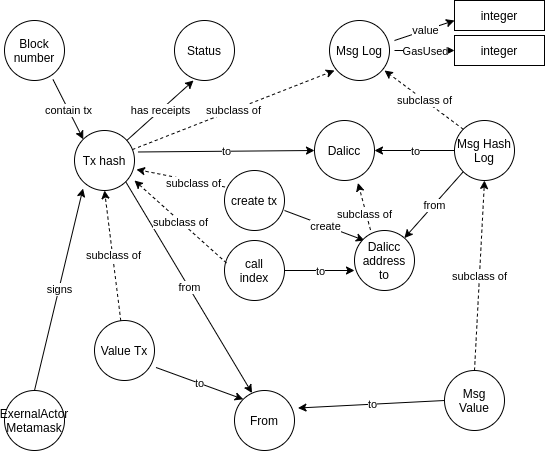
\includegraphics[width=1.45\textwidth]{images/chap03_knowledge_graph.png}
		\end{minipage}
		\caption{Transaction illustration}
		
	\end{figure}
	
\end{center}

\end{itemize}
\section{Project Architecture}
\subsection{Backend} The backend of this project rely on 2 main components: First one is the ethereum blockachain using smart contract to create platform. \\
Second one is DALICC license library is used so that user can license here/his data. In the next part, we will more focused on authenticated user as main challenge in decentralized app and data licensing system by user. 

\textbf{Authenticated user} \\
Authentication of users on Ethereum for validation purpose is the essential feature when building dApp. 
In this dApp, there are 2 ways of authentication: \\
\textit{- login to Metamask:} Metamask is the most popular cryptocurrency wallet(ethereum account) to support ethereum blockchain. additional, metamsk is bridge for web3 authentication to ethereum-based dApp. This feature would be used to offer authentication in ethereum.  \\
\textit{- Using smart contract: }the address of metamask passed to smart contract licensor, then it will
used this address as owner to license his/her file. \\

\textbf{Licensing in smart contract} \\
\textbf{License information} consists of three elements: licensor address that is passed by metamask. license of TODO\\
\textbf{Storage license information}. Each smart contract runs on ethereun blockchain would be maintain state in its permanent storage. TODO\\
\textbf{Retrieve license information}\\
As mentioned earlier, only a smart contract can change the data in its memory.
Thus, a smart contract system is validating the license requests. The JavaScript
library web3.js serves as an interface to the Ethereum Network for the frontend
of the web application. This allows the frontend to access the smart contract and
thereby retrieve license information as well as change them.TODO\\

\subsection{Front-end}
 Frontend of this project build on React.js, HTML, CSS. The React js used in this front-end for user interface.\\
 \textbf{User roadmap}\\
 The liceseing Data from user interface includes thress phases:
 \begin{itemize}
 	\item The user get asked to select to license type from which be loaded from Dalicc Library via axios get request in frontend. Then, after selecting data in next field, user should check whether there if license for selected file or data and will receive either confirmation message 'Your Data is Licensed before' or rejection message 'there is not license for this file'. 
 	\item The user should go further be pressing 'License Data/ retrieve license' button to get license information for confirmation message of the last phase or license his or her file.\\
 	license information contains some information like license type, license URI retrieved from Dalicc library and address of owner of this license. For licensing data, user get asked to login to Metamask for authentication process and this account address would be passed to smart contract as owner of this license. The licensing process will be done by receiving hash data of licensed data.
 	\item In the last Phase, user can observe receipt of this transaction in a table where contains transaction details from interaction between \textit{web3.eth} and \textit{ethOn ontology}.
 \end{itemize}
 \begin{center}
 	
 	\begin{figure}[htb!]
 		
 		\begin{minipage}{0.75\linewidth}
 			
 			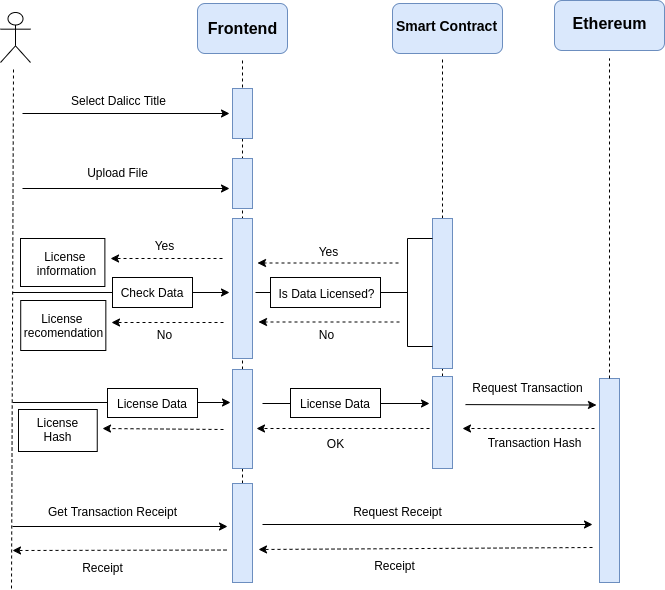
\includegraphics[width=1.45\textwidth]{images/chap03_user_roadmap.png}
 		\end{minipage}
 		\caption{DApp Architecture}
 		
 	\end{figure}
 	
 \end{center}
 \textbf{Interaction with backend}\\
 Since the backend code(smart contract) of the dApp is on decentralised network, we focused on the interaction between smart contract and thereum network. The communication between fronted and backend is taken over by Java Script library \textit{web3.js}.
 For this purpose web3 provides this connection either with HDWallet-provider to connect to test network (Sepolia in our case) or ethereum provider TODO.\\
 \textbf{interaction with with DALICC} \\
 In order to retrieve license, an HTTP GET request is sent to DALICC library endpoint and returns the license which encompasses to elements: license title and license URI. The user can choose just DALICC title as license then URI of associated title would be stored subsequently in smart contract fro further processing. 
\textbf{Produce Transaction Details}\\
After commit transaction in blockchain, user can get transaction details via web.eth, then send transaction details in RDF format to server to store into a file. The produced turtle file will be resulted into a readble format and would be return to frontend  by http GET resuest from frontend.\\
\\
\\

\subsection{Schematic Thema}
This application encompasses some components:
\begin{itemize}
	\item User interface
	\item Smart contract to communicate with DALICC library
	\item Ethereuem network to support transaction
	\item Transaction receipt
	\item EthOn ontology
	\item SPARQL query    
\end{itemize} 

\begin{center}
	
	\begin{figure}[htb!]
		
		\begin{minipage}{0.75\linewidth}
			
			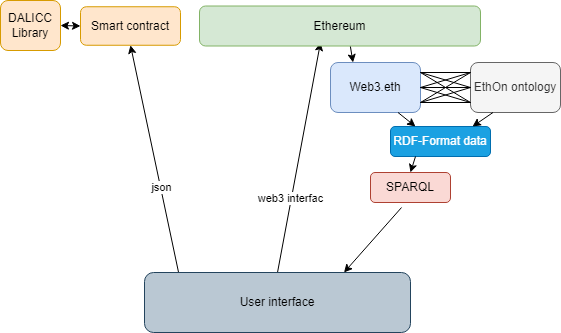
\includegraphics[width=1.5\textwidth]{images/chap03_eth_dalicc_comm.png}
		\end{minipage}
		\caption{DApp Architecture}
		
	\end{figure}
	
\end{center}

\section{Implementation}
This section comprises the implementation details in smart contract and some main functions in application.

\subsection{smart contract logic}
AS mentioned before, the backend code of this application on the ethereum network. in this section we will contemplate more on the each functionality of contract in this dApp.
\begin{itemize}
	\item \textit{Owned contract} \\
	This smart contract contains function to prevent non owner user to call function and owner as constructor to be usable in every contract which is called to. \\
	\textit{onlyOwner} \\
	This function helps us to restrict access to some function in another contract that would be called later by them. \\
	
	\item \textit{PrimaryLicenseContract} \\
	This is the main contract that communicate with two other contracts to represent public interface of licensing system.
	It provide functions to licesing data or retrieve license information. It contains two other functions as follow: \\
 	\item \textit{LicenseManager contract} \\
	THis smart contract is responsible for saving address of license or create one for new file.
	\item \textit{License contract} \\
	In this contract, the hash value and licensor address would be store here. License contract represent only one license and associate license contract for this license. The license contract should have been created by license manager.

\end{itemize}

\begin{center}
	
	\begin{figure}[htb!]
		
		\begin{minipage}{0.75\linewidth}
			
			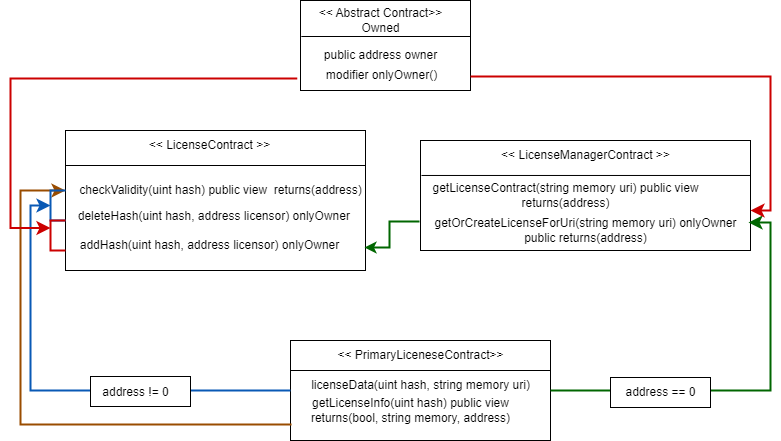
\includegraphics[width=1.45\textwidth]{images/chap03_smartContract_visual.png}
		\end{minipage}
		\caption{Smart contract visualization}
		
	\end{figure}
	
\end{center}

\text{How Smart contract works?}

\begin{itemize}
	\item \textbf{Licensing Date}
	To license data, two parameters are needed. The first one is the hash of related data and second one the address of URI of the  license.
	 This smart contract is a \textit{caller} contract
	\textit{License Data} \\
	To license data, function \textit{licenseData} is used which cecalred with two paramerters: first one is the hash of selected data, and the second one is the URI of the selected license. By pressing the 'License Data/retrieve license' on frontend, the function
	\textit{licenseData} would be triggered and  preform the steps as follow: \\
	This function checks if the target address is the zero-account, means the transaction create new contract: \\
	
	if no, \textit{deleteHash}, \\
	otherwise \textit{getOrCreateLicenseForUri}. \\
	\begin{itemize}
		\item \textit{licenseData} function check if the specified hash linked to a license and  the caller is  licensor, then \textit{deleteHash} is called and the hash of related data and address of licensor would be passed. \\
		\hspace{1cm} \textbf{Definition} \textit{deleteHash}: This function is accessible just for owner (function caller), means the caller of this function must be owner and the passed address should be licensor. Then the link between hash and license will be dropped.
		\item \textit{getOrCreateLicenseForUri} of the license Manager is called and the URI of the selected data as input parameter would be passed and returns the address to license contract which represent this URI.\\
		\hspace{1cm} \textbf{Definition} \textit{getOrCreateLicenseForUri}: This function checks if the caller of this function is owner, then exists a license contract for given URI.If so, the address of this license contract would returned. Otherwise, new licesn contarct will be created and the address of contract will be stored and returned. The caller address of the caller also will be used later as owner of this contract.
		\item \textit{addHash} function of the License contract is called with having two parameters: fist one if the hash of data , and the second one is the function caller.\\
		\hspace{1cm} \textbf{Definition} \textit{addHash}: This function is accessible just for the owner (function caller), the the link between hash value and license is created. The second parameter would be stored also as licensor. \\
		\item At the end, the event should be emitted to fire the new changes in PrimaryLicenseContarct.
		
	\end{itemize}
	\item \textbf{Change License data}
	This is doable just by licesnor  with the same way like license data.  \\
	\item \textbf{Retrieve license information}
	To retriev licnese finromation function \textit{getLicenseInfo} is called having hash of data as parameter and check if there is some license information related to this hash, then is returned the address and , otherwise, return null address and string.
	
\end{itemize}
\subsection{Forntend Workflow}
\begin{itemize}
	\item Define type:
	In this step, user get asked to select license type among many different licenses. This licenses are loaded from DALICC License Library via \textit{axios} GET request. And user must choose one of them to continue license processing.
	\item Define Content:
	In this step, the user should choose the file or data that want to be licensed. Subsequeltly, the hash \texttt{SHA3-256} of selected file is calculated which is use d to retrieve license information later.
	\item Check Your Data:
	In this step, user should check the selected data: if it is licensed beofre or not. HE/ she receives just message either confirmation 'License detected' or rejection 'NO license is detected', he or she should go further to obtain more information.
	\item License data / retrieve License information:
	Here, user receives the result of that last step, by pressing the hash value of selectd data \texttt{SHA3-256} is calculated and passed to smart contract using \textit{web.js} interface: \\
	\textbf{- } License information of the selected file or data which user received the 'license detected' message from last step. TODO more about license information
	\textbf{- } Start licensing hie /her file, if he / she received 'No license detected'  from last step. In order to license data, user get asked to log into \texttt{Metamask} to pass this account as address of licensor to smart contract. After afew second user should receive some transaction hash,  if the transaction is done successful, otherwise he/she receive the error message on frontend.
	\item Send transaction: After receiving hash of transaction in frontend , user go further to get receipt of this licensing having all details about transaction. in order to have this receipt user send transcation receipt which is not readable to server for more processing on this raw result, coverting to RDF format data and make query it to produce more readable RDF-based-data.
	\item Get Transaction receipt:
	In the last step, user can get receipt of all transaction have done till now as table in RDF format.
\end{itemize}

